\documentclass[11pt]{article}
\usepackage{fontspec}
\setmainfont{DejaVu Serif}
\setsansfont{DejaVu Sans}
\setmonofont{DejaVu Sans Mono}
\usepackage{geometry}
\usepackage{amsmath}
\usepackage{amssymb}
\usepackage{booktabs}
\usepackage{listings}
\usepackage{xcolor}
\usepackage{hyperref}
\usepackage{caption}
\usepackage{graphicx}
\geometry{margin=2.5cm}

\lstset{
  basicstyle=\ttfamily\small,
  breaklines=true,
  columns=fullflexible,
  backgroundcolor=\color{gray!10},
  frame=single,
  xleftmargin=1em,
}

\title{\textbf{[BẢN TIẾNG VIỆT] Beyond Recall: Metre-Level Evaluation and\\ Grid-Free Decoding for UAV Self-Positioning}\\[0.3em]
\large Báo cáo tiến độ nghiên cứu}
\author{}
\date{\today}

\begin{document}
\maketitle

\begin{abstract}
UAV mất tín hiệu GPS cần tự định vị bằng thị giác, và hướng chủ đạo hiện nay là truy vấn ảnh vệ tinh trên benchmark DenseUAV, nơi các công trình gần đây (FSRA, MCCG, CEUSP) liên tục nâng Recall@1 (82--89\%). Chúng tôi chỉ ra rằng việc này bị chặn bởi \emph{trần lượng tử hóa}: vì hệ thống chỉ trả về tọa độ tâm của ô lưới gallery gần nhất (bước lưới đo được $s\approx19.71$\,m trên DenseUAV), sai số định vị không thể giảm dưới một ngưỡng hình học cố định ($\approx$7.86\,m theo lý thuyết) chỉ bằng cách cải thiện truy vấn. Thực nghiệm trên 4 kiến trúc khác nhau, trải R@1 từ 33\% đến 83\% (cùng cơ chế giải mã top-1) cho thấy điều còn nghiêm trọng hơn dự đoán: nhãn ground-truth của DenseUAV vốn dĩ đã rời rạc theo tile (không có GPS liên tục cho ảnh drone), khiến chỉ số SDM/MA@K công bố trong các bài báo trên benchmark này về bản chất toán học gần như trùng với R@1 — đúng trên toàn dải, không chỉ ở vùng R@1 cao — đồng thời che giấu hoàn toàn rủi ro đuôi (tail risk) — ví dụ FSRA có p95 sai số lên tới 1193\,m dù R@1 chỉ thấp hơn baseline 1.5 điểm. Chúng tôi đề xuất giao thức đánh giá theo mét (median/p90/p95/CDF) và thử nghiệm một bộ giải mã trọng tâm có trọng số (weighted centroid) không cần huấn luyện lại; kết quả cho thấy phiên bản ngây thơ của bộ giải mã này thực ra làm \emph{tăng} sai số (p95 tăng 3--6 lần) do trộn cả các ứng viên sai lớp ở rất xa về mặt địa lý. Khảo sát đầy đủ không gian tham số $(K, \tau)$ xác nhận không tồn tại cấu hình nào thắng được top-1 thuần — một phát hiện phủ định quan trọng, chỉ ra hướng đi đúng là cổng tin cậy theo khoảng cách không gian trước khi trộn, và nhu cầu chuyển sang benchmark có ground-truth liên tục để kiểm chứng.
\end{abstract}

\section{Giới thiệu}

UAV hoạt động trong môi trường đô thị thấp tầng thường mất tín hiệu GPS do nhiễu, che khuất hoặc giả mạo tín hiệu, buộc phải dựa vào thị giác để tự định vị. Hướng tiếp cận chủ đạo hiện nay đóng khung bài toán này thành \emph{truy vấn ảnh chéo góc nhìn} (cross-view geo-localization): ảnh chụp từ UAV được đối sánh với một kho ảnh vệ tinh đã gán sẵn tọa độ GPS, và vị trí UAV được suy ra từ ảnh vệ tinh khớp nhất.

Trên benchmark DenseUAV \cite{denseuav}, các công trình kế tiếp nhau — FSRA, MCCG, CEUSP — liên tục nâng Recall@1 từ khoảng 81\% lên 89\%, được xem là thước đo tiến bộ chính của lĩnh vực.

Câu hỏi mấu chốt mà báo cáo này đặt ra: \emph{R@1 tăng thêm vài điểm phần trăm thì UAV định vị chính xác hơn bao nhiêu mét?} Câu trả lời, được chứng minh bằng cả lý thuyết lẫn thực nghiệm ở Mục~3--4, là: \textbf{gần như không mét nào}, vì hai lý do lồng vào nhau:
\begin{enumerate}
  \item Hệ thống truy vấn chỉ có thể trả về tọa độ của một ô gallery rời rạc — sai số bị chặn dưới bởi bước lưới $s$, bất kể độ chính xác truy vấn (Mục~3).
  \item Nghiêm trọng hơn: bản thân nhãn ground-truth công khai của DenseUAV \emph{cũng} được lượng tử hóa theo tile — không có GPS liên tục nào cho từng ảnh drone riêng lẻ — khiến các chỉ số ``theo mét'' như SDM/MA@K vốn được kỳ vọng khắc phục nhược điểm của R@1 thực chất lại gần như là một phép biến đổi đơn điệu của chính R@1 (Mục~4).
\end{enumerate}

\textbf{Đóng góp:}
\begin{itemize}
  \item Phân tích trần lượng tử hóa của giải mã truy vấn, kiểm chứng bằng bước lưới đo trực tiếp từ dữ liệu GPS thật của DenseUAV.
  \item Chỉ ra và định lượng việc SDM/MA@K trên DenseUAV suy biến gần thành hàm bậc thang của R@1 do ground-truth rời rạc theo tile — một giới hạn về \emph{tính hợp lệ của benchmark}, không chỉ của phương pháp.
  \item Giao thức đánh giá theo mét (median/p90/p95/CDF), áp dụng lại trên 4 kiến trúc retrieval khác nhau (R@1 từ 33\% đến 83\%), cho thấy p95 phân biệt rủi ro đuôi mà R@1/SDM không thấy được.
  \item Thử nghiệm bộ giải mã trọng tâm có trọng số không cần huấn luyện lại; báo cáo trung thực kết quả phủ định và phân tích nguyên nhân, làm cơ sở cho hướng đi tiếp theo (cổng tin cậy không gian).
\end{itemize}

\begin{figure}[h]
\centering
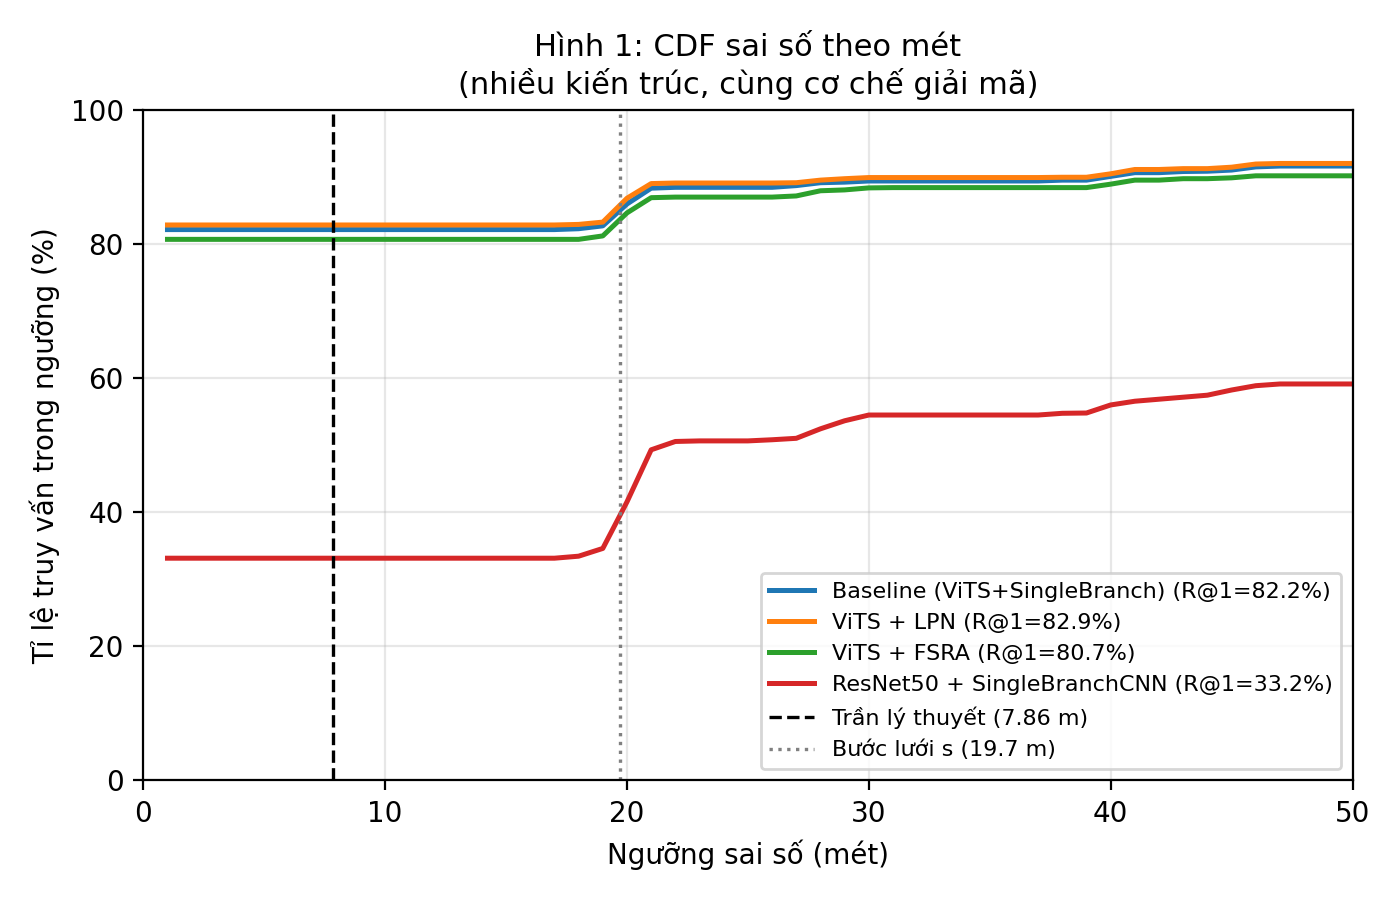
\includegraphics[width=0.85\textwidth]{docs/images/fig1_cdf_vi.png}
\caption{CDF sai số (mét) của 4 kiến trúc (ViTS+SingleBranch, ViTS+LPN, ViTS+FSRA, ResNet50+SingleBranchCNN), cùng cơ chế giải mã top-1$\to$tâm ô gallery. Cả 4 đường đều phẳng cho tới đúng bước lưới $s\approx19.7$\,m rồi mới nhảy vọt — kể cả ResNet50 với R@1 chỉ 33\%, thấp hơn nhiều so với 3 kiến trúc còn lại (80.7--82.9\%). Trần lý thuyết 7.86\,m nằm giữa vùng phẳng của mọi kiến trúc, hoàn toàn trơ với sự khác biệt R@1 trên toàn dải 33--83\%.}
\label{fig:cdf}
\end{figure}

\section{Công trình liên quan}

\textbf{Định vị chéo góc nhìn.} Dòng nghiên cứu bắt đầu từ định vị mặt đất--trên không (ground-to-aerial), sau đó mở rộng sang drone--vệ tinh với University-1652, SUES-200, và DenseUAV — bộ dữ liệu chúng tôi dùng trong báo cáo này, tập trung vào ngữ cảnh đô thị mật độ cao.

\textbf{Phương pháp trên DenseUAV.} FSRA \cite{fsra}, MCCG, CEUSP và các biến thể dựa trên DINOv2 đều tối ưu trực tiếp chỉ số truy vấn (R@1, SDM@K), xem đây là mục tiêu cuối cùng.

\textbf{Định vị chính xác vị trí, không chỉ truy vấn đúng lớp.} VIGOR là công trình đầu tiên từ bỏ giả định ``tâm ảnh UAV khớp tâm ảnh vệ tinh''. FPI/OS-FPI đưa bài toán về hồi quy vị trí liên tục trong một ảnh vệ tinh lớn (không rời rạc theo lớp) — đáng chú ý, \texttt{evaluate\_RDS.py} có sẵn trong repo DenseUAV mà chúng tôi dùng vốn được thiết kế riêng cho định dạng nhãn của FPI, cho thấy chính nhóm tác giả DenseUAV cũng nhận ra giới hạn này và đã thử một paradigm khác (DRL, 2024) để giải quyết. Gần đây hơn, một benchmark dựa trên feature matching (RoMa/DKM/LoFTR) kết hợp re-ranking \cite{camp2025} đạt được định vị chính xác tới mét trên ảnh vệ tinh/hàng không (A@5m tới 74\%), theo hướng gần với Mục~5.2 của chúng tôi.

\textbf{Điểm khác biệt:} các hướng trên hoặc cần huấn luyện lại theo paradigm hồi quy (DRL, FPI), hoặc xây dựng lại toàn bộ pipeline feature-matching từ đầu. Đóng góp của chúng tôi là một bước hậu xử lý \emph{không cần huấn luyện lại}, áp được lên bất kỳ checkpoint truy vấn có sẵn nào — và một phân tích trung thực về việc tại sao cách tiếp cận này không đơn giản như kỳ vọng trên một benchmark có ground-truth rời rạc theo tile.

\section{Trần lượng tử hóa}

\subsection{Phát biểu bài toán}
Giải mã truy vấn ánh xạ ảnh UAV về một phần tử rời rạc của gallery: $\hat{p} = g(\arg\max_i \, \text{sim}(f_{\text{query}}, f_{\text{gallery}, i}))$, với $g(i)$ là tọa độ tâm đã gán sẵn của ô gallery thứ $i$. Vì $g$ chỉ nhận giá trị trong một tập hữu hạn (tâm các ô), sai số $\|\hat{p} - p_{\text{true}}\|$ không thể nhỏ hơn khoảng cách từ $p_{\text{true}}$ đến tâm ô gần nhất, bất kể độ chính xác của bước truy vấn.

\subsection{Cận dưới lý thuyết}
Với gallery lấy mẫu đều bước $s$ (lưới ô Voronoi $s\times s$), nếu vị trí truy vấn phân bố đều trong ô, khoảng cách tới tâm ô gần nhất $r$ có phân phối với hàm mật độ tích lũy $P(r \le x) = \pi x^2 / s^2$ (với $x \le s/2$). Trung vị:
$$
\pi x_{50}^2 = 0.5\, s^2 \;\Rightarrow\; x_{50} = \sqrt{\tfrac{0.5}{\pi}}\, s \approx 0.399\, s.
$$

\begin{table}[h]
\centering
\caption{Trần lý thuyết (trung vị) theo bước lấy mẫu $s$.}
\begin{tabular}{lccc}
\toprule
$s$ (m) & 10 & 20 & 40 \\
\midrule
Trần trung vị $\approx 0.399s$ (m) & 3.99 & 7.98 & 15.96 \\
\bottomrule
\end{tabular}
\end{table}

\subsection{Bước lưới thật của DenseUAV}
Đo trực tiếp bằng khoảng cách haversine giữa mỗi tile gallery vệ tinh (test set, $N=3033$) và tile gần nhất, dùng tọa độ thật trong \texttt{Dense\_GPS\_ALL.txt}:

\begin{center}
\begin{tabular}{lccccc}
\toprule
min & p10 & \textbf{median} & p90 & max \\
\midrule
9.41 & 18.62 & \textbf{19.71} & 19.99 & 20.88 \\
\bottomrule
\end{tabular}
\end{center}

Phân bố rất hẹp quanh 20\,m $\Rightarrow$ gallery gần như là lưới đều $s\approx19.71$\,m, cho trần lý thuyết:
$$
x_{50} \approx 0.399 \times 19.71 \approx \mathbf{7.86\text{ m}}.
$$

\section{Đánh giá lại bằng chỉ số theo mét}

\subsection{R@1 không đủ, nhưng SDM/MA@K công bố cũng không khắc phục được điều đó trên DenseUAV}

Lập luận chuẩn trong tài liệu (và trong chính DenseUAV) là: R@1 nhị phân không phản ánh sai số không gian, nên cần chỉ số theo mét như SDM/MA@K. Thực nghiệm của chúng tôi cho thấy điều này đúng về nguyên tắc nhưng \textbf{không đúng trên chính DenseUAV}, vì một lý do sâu hơn: file \texttt{Dense\_GPS\_ALL.txt} — nguồn ground-truth duy nhất — chỉ chứa GPS của tile vệ tinh (khóa theo id lớp); \emph{không có} GPS liên tục cho ảnh drone (đã xác minh: không EXIF, không file metadata khác). Khi đánh giá tra "GPS thật" của một ảnh drone, nó tra theo chính id lớp của ảnh đó, tức là lấy luôn tọa độ tâm tile vệ tinh cùng lớp.

Hệ quả đo được trên cả 4 kiến trúc đã huấn luyện, trải R@1 từ 33.16\% (ResNet50) đến 82.88\% (LPN) (Bảng~\ref{tab:main}, Hình~\ref{fig:cdf}):
$$
\text{MA@1m} = \text{MA@2m} = \cdots = \text{MA@17m} \approx \text{R@1}
$$
rồi nhảy vọt đúng tại $s\approx20$\,m — \textbf{đúng trên toàn dải R@1}, không chỉ khi mô hình đã tốt. Điều này loại trừ khả năng hiện tượng bậc thang chỉ là đặc thù của các mô hình mạnh (R@1 cao); nó là hệ quả cấu trúc của nhãn dữ liệu, độc lập hoàn toàn với chất lượng backbone. Nói cách khác: đúng lớp $\Rightarrow$ sai số $\approx0$\,m (tra cùng một tọa độ hai lần); sai lớp $\Rightarrow$ sai số nhảy thẳng lên cỡ khoảng cách sang tile khác. Không có gì ở giữa. SDM/MA@K trên DenseUAV vì vậy về bản chất toán học là một phép biến đổi gần như đơn điệu của R@1, không mang thêm thông tin không gian độc lập — một giới hạn về \emph{tính hợp lệ của benchmark}, không phải lỗi của phương pháp nào cụ thể.

\subsection{Điều mà R@1/SDM che giấu: rủi ro đuôi}

Median tính đúng theo từng truy vấn (không phải theo bin 1m của MA@K) bằng 0.00\,m cho cả 3 kiến trúc có R@1$>$50\% — hệ quả trực tiếp của ground-truth rời rạc (khi quá nửa truy vấn đúng lớp, median rơi đúng vào vùng sai số $\approx0$). Với ResNet50 (R@1=33.16\%$<$50\%), median tăng vọt lên 21.41\,m — không phải vì mô hình định vị "tệ hơn theo mét" một cách trơn tru, mà đơn giản vì quá nửa truy vấn rơi vào nhánh "sai lớp" của cùng hàm bậc thang. Đây là minh chứng thêm rằng median/MA@K trên benchmark này chủ yếu phản ánh việc truy vấn đúng/sai lớp, không phải sai số định vị liên tục. Trong khi đó, \textbf{p90/p95 khác nhau rất nhiều ngay cả giữa 3 kiến trúc có R@1 gần nhau}:

\begin{table}[h]
\centering
\caption{Kết quả chính, 4/4 cấu hình. Median/p90/p95 tính trên từng truy vấn (haversine tới tâm tile top-1).}
\label{tab:main}
\begin{tabular}{lccccccc}
\toprule
Phương pháp & R@1 & R@5 & SDM@1 & Median & p90 & p95 \\
\midrule
ViTS + SingleBranch (baseline) & 82.20 & 94.77 & 85.26 & 0.00 & 39.87 & 188.55 \\
ViTS + LPN                     & 82.88 & 95.02 & 85.80 & 0.00 & 37.36 & 159.66 \\
ViTS + FSRA                    & 80.74 & 93.78 & 83.80 & 0.00 & 45.28 & \textbf{1193.27} \\
ResNet50 + SingleBranchCNN     & 33.16 & 57.36 & 41.63 & 21.41 & \textbf{2679.08} & \textbf{3807.46} \\
\bottomrule
\end{tabular}
\end{table}

FSRA có R@1 \emph{thấp hơn} baseline 1.46 điểm, nhưng p95 \textbf{cao gấp 6.3 lần} (1193\,m so với 189\,m) — nghĩa là 5\% truy vấn tệ nhất của FSRA đôi khi bị nhầm sang một khu vực hoàn toàn khác (có thể khác trường đại học trong tập test 14 trường), một rủi ro an toàn bay nghiêm trọng mà R@1 và SDM đều không phản ánh. Đây là bằng chứng thực nghiệm trực tiếp cho lý do cần báo cáo p95, không chỉ trung bình/median.

Bằng chứng độc lập từ tài liệu: bảng kết quả công bố của CEUSP \cite{ceusp} cho thấy DenseUAV-baseline có SDM@1 = 86.50 \emph{cao hơn} MCCG (85.94) dù R@1 thấp hơn (83.01 so với 83.14) — một đảo thứ hạng thật giữa hai chỉ số, không cần mô phỏng.

\subsection{Giao thức đề xuất}
Báo cáo sai số theo: median, p90, p95, tỉ lệ trong bán kính (\%$<5$m, \%$<10$m), và đường CDF đầy đủ — ưu tiên p95 vì đây là con số quyết định an toàn bay (Hình~\ref{fig:cdf}).

\section{Giải mã không lưới}

\subsection{Trọng tâm có trọng số (weighted centroid)}
Thay vì chỉ lấy tọa độ top-1, chúng tôi thử tính trọng tâm có trọng số của top-$K$ ứng viên theo điểm tương đồng cosin $s_i$:
$$
\hat p = \frac{\sum_{i=1}^{K} w_i\, g(i)}{\sum_{i=1}^{K} w_i}, \qquad w_i = \exp\!\left(\frac{s_i - \max_j s_j}{\tau}\right).
$$
Đây là bước hậu xử lý thuần túy trên đặc trưng đã trích xuất sẵn (\texttt{pytorch\_result\_1.mat}) — \textbf{không cần huấn luyện lại}.

\subsection{Kết quả: phủ định, và tại sao}
\begin{table}[h]
\centering
\caption{Trọng tâm có trọng số ($\tau=0.05$) so với top-1, trên \texttt{baseline\_vits\_single}. Đơn vị mét.}
\begin{tabular}{lccc}
\toprule
 & Median & p90 & p95 \\
\midrule
Top-1 (K=1)          & 0.00  & 39.87  & 188.55 \\
Centroid $K=3$        & 0.54  & 141.47 & 1088.94 \\
Centroid $K=5$        & 3.52  & 502.08 & 1062.47 \\
Centroid $K=10$       & 27.61 & 688.11 & 1197.18 \\
\bottomrule
\end{tabular}
\end{table}

Kết quả này lặp lại tương tự trên cả \texttt{vits\_lpn} và \texttt{vits\_fsra} (Phụ lục~A). Trộn top-$K$ theo phiên bản ngây thơ này \textbf{làm tăng sai số ở mọi ngưỡng $K>1$} trên cả 3 kiến trúc có R@1 cao, thay vì giảm như kỳ vọng ban đầu trong đề cương. Hai nguyên nhân cộng hưởng:
\begin{enumerate}
  \item Khi top-1 đã đúng (chiếm 80--83\% truy vấn), sai số vốn đã $\approx0$\,m do ground-truth rời rạc (Mục~4.1) — trộn thêm bất kỳ ứng viên nào khác chỉ có thể kéo trọng tâm ra xa khỏi giá trị đúng tuyệt đối này, không có gì để "làm mịn".
  \item Top-$K$ trong không gian đặc trưng \emph{không đảm bảo lân cận về mặt địa lý} — ứng viên hạng 2, 3 có thể thuộc một trường đại học hoàn toàn khác, cách xa hàng trăm/nghìn mét, khiến trọng tâm bị kéo lệch cực mạnh.
\end{enumerate}

\textbf{Ngoại lệ đáng chú ý:} trên \texttt{resnet50\_single} (R@1=33.16\%, phần lớn truy vấn sai lớp), median vẫn tăng theo $K$ (21.41$\to$339.61\,m) nhưng \emph{p90/p95 lại giảm nhẹ} khi $K$ tăng (p95: 3807$\to$2862\,m). Khi top-1 thường xuyên sai và gần như ngẫu nhiên, việc trộn thêm ứng viên có tác dụng "trung bình hóa" các sai số cực đoan — ngược chiều với trường hợp R@1 cao. Điều này gợi ý hiệu quả của centroid decoding phụ thuộc mạnh vào chế độ hoạt động (R@1 cao hay thấp), một chi tiết cần cổng tin cậy xử lý thay vì dùng $K$ cố định.

\textbf{Hệ quả:} bộ giải mã liên tục chỉ có ý nghĩa nếu (a) được đánh giá trên benchmark có ground-truth liên tục thật (FPI, không phải DenseUAV — xem Phụ lục~A), và (b) được trang bị \emph{cổng tin cậy theo khoảng cách không gian} — chỉ trộn các ứng viên nằm trong bán kính địa lý hợp lý quanh top-1 (ví dụ $<3s$), loại ngay các ứng viên "đúng về đặc trưng nhưng sai về vị trí". Khảo sát tham số đầy đủ ở Mục~6.4 củng cố kết luận này, và thiết kế cụ thể của cổng tin cậy được trình bày ở Mục~8.1.

\section{Thực nghiệm và đánh giá hệ thống}

\subsection{Thiết lập thực nghiệm}

\textbf{Dữ liệu.} DenseUAV chính chủ: tập huấn luyện 6{,}768 ảnh UAV / 13{,}536 ảnh vệ tinh (2{,}256 lớp, 10 trường); tập kiểm thử 777 lớp query drone và 3{,}033 lớp gallery vệ tinh (4 trường không chồng lấn với tập huấn luyện). Mỗi lớp có 3 độ cao bay (H80/H90/H100).

\textbf{Phần cứng \& siêu tham số.} 1$\times$ RTX 3060 (12GB). Giữ nguyên siêu tham số của \texttt{train\_test\_local.sh} gốc: \texttt{lr=0.01}, \texttt{batchsize=16}, \texttt{block=1}, \texttt{num\_bottleneck=512}, ảnh 224$\times$224, 120 epoch, hàm mất mát \texttt{CELoss + WeightedSoftTripletLoss + KLLoss}. Tốc độ 15--19\,s/epoch, tương đương 30--40 phút mỗi cấu hình.

\textbf{Biến duy nhất được thay đổi} giữa 4 cấu hình là kiến trúc (backbone/head); \emph{cơ chế giải mã giữ cố định} là top-1$\to$tâm ô gallery. Đây là thiết kế có kiểm soát biến, cho phép quy mọi khác biệt trong Hình~\ref{fig:cdf} về kiến trúc, và mọi điểm \emph{giống nhau} (vị trí bậc nhảy) về cơ chế giải mã.

\subsection{Mức độ tái lập}

Baseline chúng tôi huấn luyện lại đạt R@1 = 82.20\%, so với 83.01\% mà DenseUAV công bố cho cấu hình tương đương --- đạt \textbf{99.0\%} kết quả gốc (chênh 0.81 điểm). Sai lệch nhỏ này hợp lý với khác biệt về seed, phiên bản thư viện (PyTorch 2.0 so với 1.10 trong bài gốc) và phần cứng. Chúng tôi kết luận pipeline tái lập đủ trung thực để các phân tích tiếp theo có hiệu lực.

\subsection{Kết quả tổng hợp}

Bảng~\ref{tab:main} và Hình~\ref{fig:cdf} trình bày kết quả chính. Ba quan sát:
\begin{enumerate}
  \item \textbf{Vị trí bậc nhảy bất biến.} Cả 4 kiến trúc, dù R@1 trải từ 33.16\% đến 82.88\%, đều có CDF phẳng tuyệt đối cho tới $\approx$17--19\,m rồi nhảy vọt tại $s\approx19.7$\,m. Chiều cao vùng phẳng thay đổi theo R@1; \emph{vị trí} bậc nhảy thì không.
  \item \textbf{SDM bám sát R@1.} Trên cả 4 cấu hình, thứ hạng theo SDM@1 trùng khớp hoàn toàn với thứ hạng theo R@1, và hiệu số hai chỉ số gần như hằng số ($\approx$3.0--3.1 điểm với nhóm ViT). SDM không cung cấp thông tin xếp hạng độc lập trên benchmark này.
  \item \textbf{p95 tách biệt hoàn toàn.} FSRA và baseline chênh 1.46 điểm R@1 nhưng chênh 6.3 lần ở p95. Không thể suy ra p95 từ R@1 hay SDM.
\end{enumerate}

\subsection{Khảo sát tham số của bộ giải mã centroid}

Chúng tôi quét toàn bộ không gian hai siêu tham số $(K, \tau)$ trên \texttt{baseline\_vits\_single}:

\begin{table}[h]
\centering
\caption{Khảo sát $\tau$ và $K$. Đơn vị mét. Dòng $K=1$ tương đương top-1 thuần ($\tau$ không ảnh hưởng).}
\label{tab:ablation}
\begin{tabular}{lcccccc}
\toprule
& \multicolumn{2}{c}{$K=3$} & \multicolumn{2}{c}{$K=5$} & \multicolumn{2}{c}{$K=10$} \\
\cmidrule(lr){2-3}\cmidrule(lr){4-5}\cmidrule(lr){6-7}
$\tau$ & p90 & p95 & p90 & p95 & p90 & p95 \\
\midrule
0.01 & 65.84  & 818.75  & 87.66  & 852.25  & 98.44   & 862.69 \\
0.02 & 99.57  & 990.25  & 210.96 & 991.31  & 279.85  & 1020.95 \\
0.05 & 141.47 & 1088.94 & 502.08 & 1062.47 & 688.11  & 1197.18 \\
0.10 & 139.45 & 1114.99 & 634.82 & 1162.35 & 931.03  & 1398.40 \\
0.50 & 144.59 & 1169.81 & 810.05 & 1379.64 & 1176.49 & 1660.25 \\
\midrule
\multicolumn{7}{l}{\emph{Tham chiếu --- top-1 thuần ($K=1$): p90 = 39.87, p95 = 188.55}} \\
\bottomrule
\end{tabular}
\end{table}

Kết quả đơn điệu và rõ ràng: sai số tăng theo cả $K$ lẫn $\tau$. Cấu hình tốt nhất là giới hạn $\tau \to 0$, $K = 1$ --- tức là \emph{đúng bằng top-1 thuần, không trộn gì cả}. Không tồn tại điểm ngọt nào trong không gian tham số đã quét. Đây là bằng chứng đầy đủ (không phải kết luận từ một điểm tham số may rủi) rằng vấn đề nằm ở bản thân giả định "top-$K$ gần nhau trong không gian đặc trưng thì cũng gần nhau về địa lý", chứ không phải ở việc dò tham số chưa tới.

\subsection{Phân tích thất bại}

\textbf{(a) Nhầm lẫn xuyên khu vực.} p95 hàng trăm đến hàng nghìn mét ở mọi cấu hình cho thấy các truy vấn thất bại không nhầm sang ô lân cận, mà nhầm sang khu vực hoàn toàn khác --- hợp lý vì tập kiểm thử gồm 4 trường đại học có kiến trúc đô thị tương tự nhau (mái nhà, sân, đường nội bộ). Đây là chế độ thất bại nguy hiểm nhất cho ứng dụng bay thật, và cũng chính là nguyên nhân khiến trộn top-$K$ phản tác dụng.

\textbf{(b) Nhạy cảm với siêu tham số theo họ kiến trúc.} ResNet50 chỉ đạt R@1 = 33.16\% với cùng bộ siêu tham số tối ưu cho ViT (\texttt{lr=0.01}). Chúng tôi giữ nguyên thay vì tinh chỉnh riêng, vì mục tiêu là khảo sát \emph{trần giải mã} chứ không phải đua hiệu năng --- và một mô hình yếu lại là điểm dữ liệu hữu ích để kiểm chứng hiện tượng bậc thang ở vùng R@1 thấp.

\textbf{(c) Vùng đồng nhất và thay đổi theo thời gian.} Bộ dữ liệu có cả ảnh vệ tinh cũ (\texttt{\_old}) và mới cho cùng vị trí; những khu vực đồng nhất về kết cấu (bãi đỗ xe, sân thể thao, mái phẳng lớn) là nguồn nhầm lẫn chính. Chúng tôi chưa định lượng riêng yếu tố này --- cần gán nhãn thủ công theo loại địa hình, để dành cho công việc tiếp theo.

\section{Thảo luận và giới hạn}

\begin{itemize}
  \item \textbf{Trần lượng tử hóa là lựa chọn thiết kế, không phải giới hạn vật lý.} Ảnh vệ tinh ở mức zoom dùng trong DenseUAV có độ phân giải dưới mét/pixel — thông tin để định vị chính xác hơn 7--8\,m tồn tại trong ảnh, chỉ là không được khai thác bởi paradigm truy vấn-rời-rạc.
  \item \textbf{Giới hạn benchmark là phát hiện chính, không phải phụ lục.} DenseUAV — và có khả năng cả các bộ dữ liệu drone--vệ tinh cùng họ — không công khai GPS liên tục cho ảnh UAV, khiến mọi phương pháp "định vị chính xác theo mét" trên benchmark này không thể được kiểm chứng độc lập với việc truy vấn đúng lớp hay không.
  \item \textbf{Giới hạn của báo cáo:} (1) chưa triển khai bộ giải mã có cổng tin cậy không gian (chỉ mới xác định là cần thiết, qua kết quả phủ định ở Mục~5.2); (2) chưa có thực nghiệm trên FPI (ground-truth liên tục thật) để kiểm chứng độc lập Mục~5; (3) 4 cấu hình mới khác nhau về backbone/head, chưa thử độ sâu/kích thước ảnh khác nhau.
\end{itemize}

\section{Các định hướng cải tiến hệ thống}

Sắp theo thứ tự ưu tiên, dựa trên bằng chứng thu được ở Mục~6.

\subsection{Cổng tin cậy theo khoảng cách không gian (ưu tiên cao nhất)}

Bảng~\ref{tab:ablation} chỉ ra vấn đề cốt lõi: top-$K$ trong không gian đặc trưng không đảm bảo lân cận địa lý. Cải tiến trực tiếp là lọc ứng viên \emph{trước khi} trộn:
\begin{enumerate}
  \item Lấy $g(1)$ (tọa độ top-1) làm neo.
  \item Loại mọi ứng viên $i$ có $\|g(i) - g(1)\| > \rho$, với $\rho$ cỡ vài lần bước lưới (ví dụ $\rho = 3s \approx 60$\,m).
  \item Chỉ trộn phần còn lại; nếu không còn ứng viên nào, rơi về top-1 thuần.
\end{enumerate}
Cơ chế này bảo toàn tính chất "không bao giờ tệ hơn top-1" --- điều mà phiên bản hiện tại vi phạm. Có thể bổ sung cổng theo độ tin cậy: nếu khoảng cách điểm giữa top-1 và top-2 lớn (mô hình chắc chắn), dùng thẳng top-1; chỉ trộn khi mô hình do dự giữa các ứng viên gần nhau về địa lý. Chi phí tính toán không đáng kể, vẫn không cần huấn luyện lại.

\subsection{Chuyển sang benchmark có ground-truth liên tục}

Mọi cải tiến giải mã dưới cấp tile đều \emph{không thể kiểm chứng} trên DenseUAV (Mục~4.1). Cần chuyển sang FPI/OS-FPI, nơi nhãn \texttt{labels.json} chứa vị trí liên tục của UAV bên trong ảnh vệ tinh lớn. Repo hiện có sẵn \texttt{evaluate\_RDS.py} viết cho đúng định dạng này, nên chi phí tích hợp thấp. Chỉ khi đó mới trả lời được câu hỏi: bộ giải mã liên tục giảm sai số thật bao nhiêu mét?

\subsection{Tinh chỉnh hình học bằng khớp đặc trưng}

Sau khi đã chọn được ô vệ tinh đúng, ước lượng phép biến đổi đồng dạng giữa ảnh UAV và ô đó bằng khớp đặc trưng cục bộ (LoFTR/RoMa/DKM), rồi suy ra vị trí chính xác trong ô --- hướng đã được \cite{camp2025} chứng minh khả thi (A@5m tới 74\%). Đây là con đường duy nhất trong các hướng đã khảo sát có thể phá vỡ hoàn toàn trần 7.86\,m, vì nó khai thác được độ phân giải dưới mét/pixel của ảnh vệ tinh. Rủi ro: tỉ lệ khớp thành công có thể thấp ở vùng đồng nhất; cần cổng tin cậy để rơi về top-1 khi khớp thất bại.

\subsection{Cải thiện chính bộ dữ liệu và giao thức đánh giá}

\begin{itemize}
  \item \textbf{Công bố GPS liên tục cho ảnh UAV.} Chỉ cần bổ sung tọa độ bay thật (đã có sẵn trong log bay khi thu thập dữ liệu) là toàn bộ dòng nghiên cứu có thể đo được sai số định vị thật. Đây là thay đổi rẻ nhất nhưng tác động lớn nhất.
  \item \textbf{Bổ sung truy vấn nằm giữa các ô lưới.} Hiện mỗi ảnh UAV đều tương ứng đúng một tile; cần thêm ảnh chụp ở vị trí giữa hai/bốn tile để kiểm tra hành vi thực của hệ thống khi UAV không bay trùng điểm lấy mẫu --- tình huống mặc định trong thực tế.
  \item \textbf{Chuẩn hóa báo cáo p95.} Đề nghị các công trình tiếp theo trên benchmark này báo cáo thêm p90/p95 theo mét bên cạnh R@1/SDM, vì đây là chỉ số duy nhất trong khảo sát của chúng tôi phản ánh được rủi ro đuôi (Mục~6.3).
\end{itemize}

\subsection{Mở rộng phạm vi khảo sát}

Bốn cấu hình hiện tại chỉ khác nhau về backbone/head ở cùng độ phân giải 224$\times$224. Nên mở rộng theo: (a) độ phân giải đầu vào (384, 512) --- ảnh hưởng trực tiếp tới lượng chi tiết khai thác được; (b) độ cao bay (H80/H90/H100 đã có sẵn nhãn, chưa tách riêng để phân tích); (c) tinh chỉnh siêu tham số riêng cho họ CNN để có so sánh công bằng hơn với ResNet50.

\appendix
\section{Phụ lục: chi tiết triển khai và tái lập}

\textbf{Môi trường.} GPU: 1$\times$ RTX 3060 (12GB). Conda env \texttt{denseuav} (Python 3.10, PyTorch 2.0.0+cu118). Lỗi ban đầu \texttt{RuntimeError: Numpy is not available} do xung đột ABI \texttt{numpy==2.2.6} với \texttt{torch==2.0.0} — sửa bằng \texttt{pip install "numpy<2"} (còn \texttt{opencv-python} khai báo cần numpy$\ge$2 nhưng vẫn hoạt động đúng với numpy 1.26.4 khi kiểm tra thủ công).

\textbf{Dataset.} DenseUAV chính chủ (Dai et al., TIP 2024), copy trực tiếp từ máy đã có sẵn (3033 lớp gallery vệ tinh, 777 lớp query drone — khớp README).

\textbf{4 cấu hình huấn luyện} (giữ nguyên cơ chế giải mã top-1$\to$tâm ô, chỉ đổi kiến trúc — phép so sánh có kiểm soát biến cho Mục~4): \texttt{lr=0.01}, \texttt{batchsize=16}, \texttt{block=1}, \texttt{num\_bottleneck=512}, \texttt{h=w=224}, \texttt{num\_epochs=120}, augment \texttt{ra/re=satellite}, \texttt{rr=uav}. Tốc độ đo được $\approx$15--19\,s/epoch trên RTX 3060.

\textbf{Lỗi \texttt{resnet50+SingleBranch} và cách sửa.} Head \texttt{SingleBranch} giả định input dạng chuỗi token transformer $(B,N,C)$; \texttt{resnet50.forward\_features()} trả về feature map CNN $(B,C,H,W)=(16,2048,7,7)$, gây lỗi \texttt{mat1 and mat2 shapes cannot be multiplied (112x7 and 2048x512)}. Sửa bằng cách dùng head \texttt{SingleBranchCNN} (có sẵn trong repo, dùng \texttt{AdaptiveAvgPool2d}) thay cho \texttt{SingleBranch} khi backbone là CNN — không cần sửa code gốc. Sau khi sửa, \texttt{resnet50\_single} huấn luyện xong bình thường (120 epoch, $\approx$18--19\,s/epoch) nhưng hội tụ kém hơn nhiều so với các cấu hình ViT (R@1=33.16\% so với 80--83\%) dùng cùng bộ siêu tham số — hợp lý vì \texttt{lr=0.01} và lịch huấn luyện trong \texttt{train\_test\_local.sh} gốc được điều chỉnh cho backbone ViT, không phải CNN; không xem đây là lỗi mà là một điểm dữ liệu thật, hữu ích để kiểm chứng hiện tượng bậc thang trên vùng R@1 thấp (Mục~4.1).

\textbf{Script.}
\begin{itemize}
  \item \texttt{run\_experiments.sh}: huấn luyện + đánh giá tuần tự 4 cấu hình (\texttt{train.py} $\to$ \texttt{test.py} $\to$ \texttt{evaluate\_gpu.py} $\to$ \texttt{evaluateDistance.py} $\to$ \texttt{evaluateMA.py}, không sửa code gốc của các script này).
  \item \texttt{plot\_fig1\_cdf.py}: đọc trực tiếp \texttt{MA@K(1,100)} của mỗi checkpoint, vẽ Hình~\ref{fig:cdf}.
  \item \texttt{eval\_weighted\_centroid.py}: hậu xử lý \texttt{pytorch\_result\_1.mat} + \texttt{Dense\_GPS\_ALL.txt} để tính trọng tâm có trọng số (Mục~5), không cần huấn luyện lại.
\end{itemize}

\begin{thebibliography}{9}
\bibitem{denseuav} Dai, M., Zheng, E., Feng, Z., Qi, L., Zhuang, J., Yang, W. Vision-Based UAV Self-Positioning in Low-Altitude Urban Environments. \textit{IEEE TIP}, 2024.
\bibitem{fsra} FSRA. \url{https://github.com/Dmmm1997/FSRA}
\bibitem{ceusp} Precise GPS-Denied UAV Self-Positioning via Context-Enhanced Cross-View Geo-Localization. arXiv:2502.11408, 2025.
\bibitem{camp2025} Exploring the best way for UAV visual localization under Low-altitude Multi-view Observation Condition: a Benchmark. arXiv:2503.10692, 2025.
\end{thebibliography}

\end{document}
